\subsection{Synchroniser}

\begin{figure}[htbp]
   \centering
   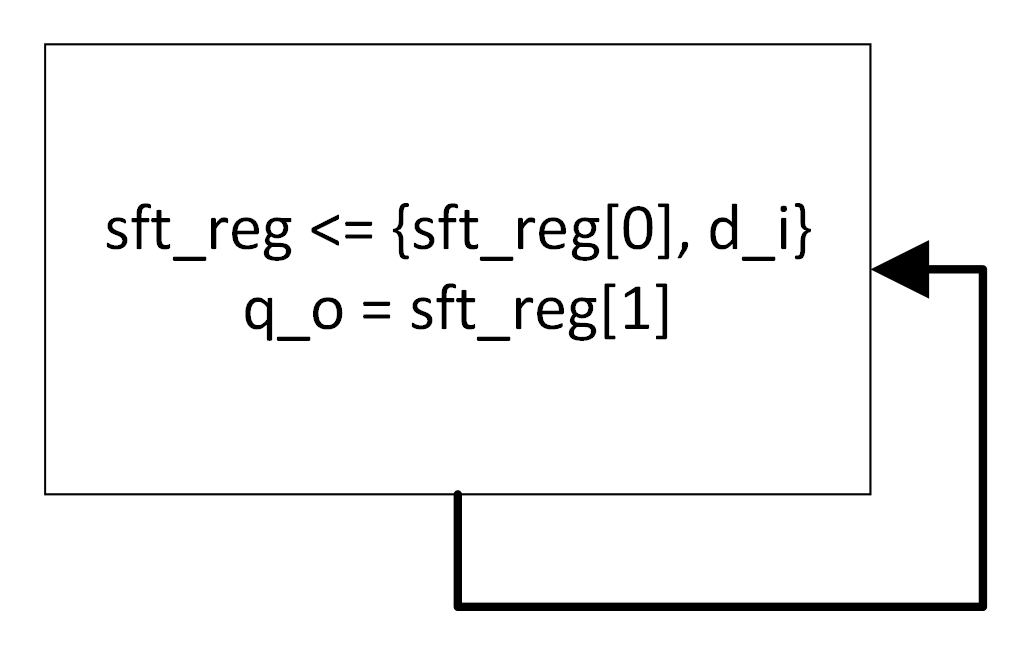
\includegraphics[width=0.5\textwidth]{synchroniser_asm.png}
   \caption{ASM chart of the synchroniser module.}
   \label{fig:synchroniser_asm}
\end{figure}

\begin{minted}[
   fontsize=\footnotesize,
   linenos,
   breaklines,
]{verilog}
module sync (
   input clk_i,
   input d_i,
   output q_o
);

reg [1:0] sft_reg;

always@(posedge clk_i)
   sft_reg <= {sft_reg[0], d_i};

assign q_o = sft_reg[1];

endmodule
\end{minted}

\begin{minted}[
   fontsize=\footnotesize,
   linenos,
   breaklines,
]{verilog}
module sync_tb;

// Inputs
reg clk;
reg d_i;

// Outputs
wire q_o;

sync DUT (
   .clk_i(clk),
   .d_i(d_i),
   .q_o(q_o)
);

// Create a 50Mhz clock
always #10 clk = !clk;  // every ten nanoseconds invert

initial begin
   clk = 1'b0;
   d_i = 1'b1;
end

initial begin
   #20;

   // Long press
   #16;
   d_i = 1'b0;
   #43;
   d_i = 1'b1;

   // Brief contact
   #46;
   d_i = 1'b0;
   #3;
   d_i = 1'b1;
   #20;

   // Long press after brief contact
   #16;
   d_i = 1'b0;
   #43;
   d_i = 1'b1;
   #100;

// Finish the Simulation
   #100;
   $finish;
end

endmodule
\end{minted}

\begin{figure}[htbp]
   \centerline{
   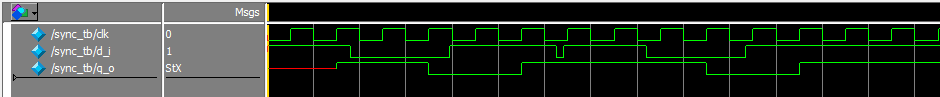
\includegraphics[width=\paperwidth]{synchroniser_sim.png}}
   \caption{Testbench simulation of the synchroniser module.}
   \label{fig:synchroniser_sim}
\end{figure}

Fig.~\ref{fig:synchroniser_sim} displays the simulation test results of the synchroniser module. The synchroniser delayed input signal by two clock cycle and aligned the edge of the input signal with the clock edges. Short signals may be ignored by the synchroniser.
